The high computational cost of high-fidelity codes often precludes direct Monte Carlo simulations, necessitating the use of surrogate models, also known as emulators. While Gaussian Processes~(GP) and Polynomial Chaos Expansions~(PCE) are standard for deterministic systems, they cannot be directly applied to stochastic simulators where a single evaluation is insufficient to characterize the output distribution.

Mathematically, a stochastic simulator $\mathcal{M}_S$ can be viewed as a mapping that incorporates deterministic variables and inherent randomness. For a given vector of input parameters $\mathbf{x}$ within the domain $\mathcal{D}_X$, the output is not a single deterministic value, but a random variable $Y_{\mathbf{x}}$. This relationship is formally expressed as:

\begin{equation}\mathcal{M}_S : \mathcal{D}_X \times \Omega \rightarrow \mathbb{R}, \qquad(\mathbf{x}, \omega) \mapsto \mathcal{M}_S(\mathbf{x}, \omega),\end{equation}

In this formulation, $\mathbf{x}$ represents the set of controlled input parameters (e.g., geometry, material properties), while $\omega$ denotes a random event from the probability space $\Omega$. This latent variable $\omega$ introduces the stochasticity into the system. Consequently, for a fixed input $\mathbf{x}$, the simulator produces a distribution of possible outcomes rather than a unique solution.

In the context of durability assessment of reinforced concrete, the carbonation process is influenced by several sources of uncertainty, ranging from material heterogeneity to environmental fluctuations. To effectively capture these complex probabilistic behaviors without the computational cost of exhaustive simulations, this study employs the Generalized Lambda Distribution (GLD) as a stochastic emulator. The GLD is a highly flexible four-parameter distribution family designed to approximate a wide range of parametric distributions \cite{KarianDudewicz2000, ZhuSudret2020-GLAMoriginal}.

The Generalized Lambda Distribution (GLD) is defined by its \textit{quantile function} $Q(u)$, which is the inverse of the Cumulative Distribution Function (CDF), i.e., $Q(u) = F^{-1}(u)$. This approach is particularly advantageous for stochastic emulation as it facilitates the inverse transform sampling method. In this study, we consider the Freimer-Kollia-Mudholkar-Lin (FKML) family \cite{Freimer1988}, which is defined as:

\begin{equation}
Q(u) = \lambda_1 + \frac{1}{\lambda_2} \left( \frac{u^{\lambda_3} - 1}{\lambda_3} - \frac{(1 - u)^{\lambda_4} - 1}{\lambda_4} \right)
\label{eq:GLD_quantile}
\end{equation}

where $u \in [0, 1]$ represents the cumulative probability. The distribution is governed by four parameters: $\lambda_1$ is the \textit{location} parameter, $\lambda_2$ is the \textit{scaling} parameter (with the requirement $\lambda_2 > 0$), and $\lambda_3, \lambda_4$ are the \textit{shape} parameters.

\subsection{Parameter Estimation via Method of Moments}

To calibrate the GLD emulator, the four parameters $\boldsymbol{\lambda} = \{\lambda_1, \dots, \lambda_4\}$ must be estimated from a set of model evaluations \cite{chalabi2011gld,karian2010handbook,corlu2016estimating} . In this study, we employ the \textit{Method of Moments} (MoM) \cite{lakhany2000estimating}, which consists of matching the theoretical moments of the GLD to the empirical moments computed from the sample set $\mathcal{Y} = \{y^{(1)}, \dots, y^{(N)}\}$. The first four central moments, namely the mean $\mu$, variance $\sigma^2$, skewness $\delta$, and kurtosis $\kappa$, are analytically related to the $\lambda$-parameters as follows:

\begin{align}
\mu &= \lambda_1 - \frac{1}{\lambda_2} \left( \frac{1}{\lambda_3 + 1} - \frac{1}{\lambda_4 + 1} \right) \label{eq:mean} \\
\sigma^2 &= \frac{v_2 - v_1^2}{\lambda_2^2} \label{eq:var} \\
\delta &= \frac{v_3 - 3v_1v_2 + 2v_1^3}{(v_2 - v_1^2)^{3/2}} \label{eq:skew} \\
\kappa &= \frac{v_4 - 4v_1v_3 + 6v_1^2v_2 - 3v_1^4}{(v_2 - v_1^2)^2} \label{eq:kurt}
\end{align}

In these expressions, $v_k$ denotes a non-linear function that depends solely on $\lambda_3$ and $\lambda_4$. In Eq.~\eqref{eq:vk}, $B(\cdot, \cdot)$ represents the Beta function, defined as:

\begin{equation}
v_k = \sum_{j=0}^{k} \frac{(-1)^j}{\lambda_3^{k-j} \lambda_4^j} \binom{k}{j} B(\lambda_3(k-j) + 1, \lambda_4j + 1) \label{eq:vk}
\end{equation}

The calibration of the GLD parameters is formulated as an inverse problem, where the objective is to minimize the discrepancy between the analytical moments (Eqs. \ref{eq:mean}--\ref{eq:kurt}) and the empirical moments derived from the stochastic simulator. To solve this non-linear system, the Broyden-Fletcher-Goldfarb-Shanno (BFGS) optimization algorithm was employed \cite{nocedal2006}. BFGS is a quasi-Newton method particularly suited for this type of parameter estimation due to its efficient handling of gradients and convergence properties in multi-dimensional spaces\cite{broyden1965}. The numerical procedure was implemented using PyGLAM, an in-house Python library specifically developed for the emulation of stochastic simulators using Generalized Lambda Distributions.

Using PyGLAM, Figure~\ref{fig:pyglam_fits} shows examples of fitting the GLD to traditional distributions such as the Normal, Gumbel, and Uniform.

\begin{figure}[htbp]
     \centering
     % --- Primeira Subfigura (Normal) ---
     \begin{subfigure}[b]{0.32\textwidth}
         \centering
         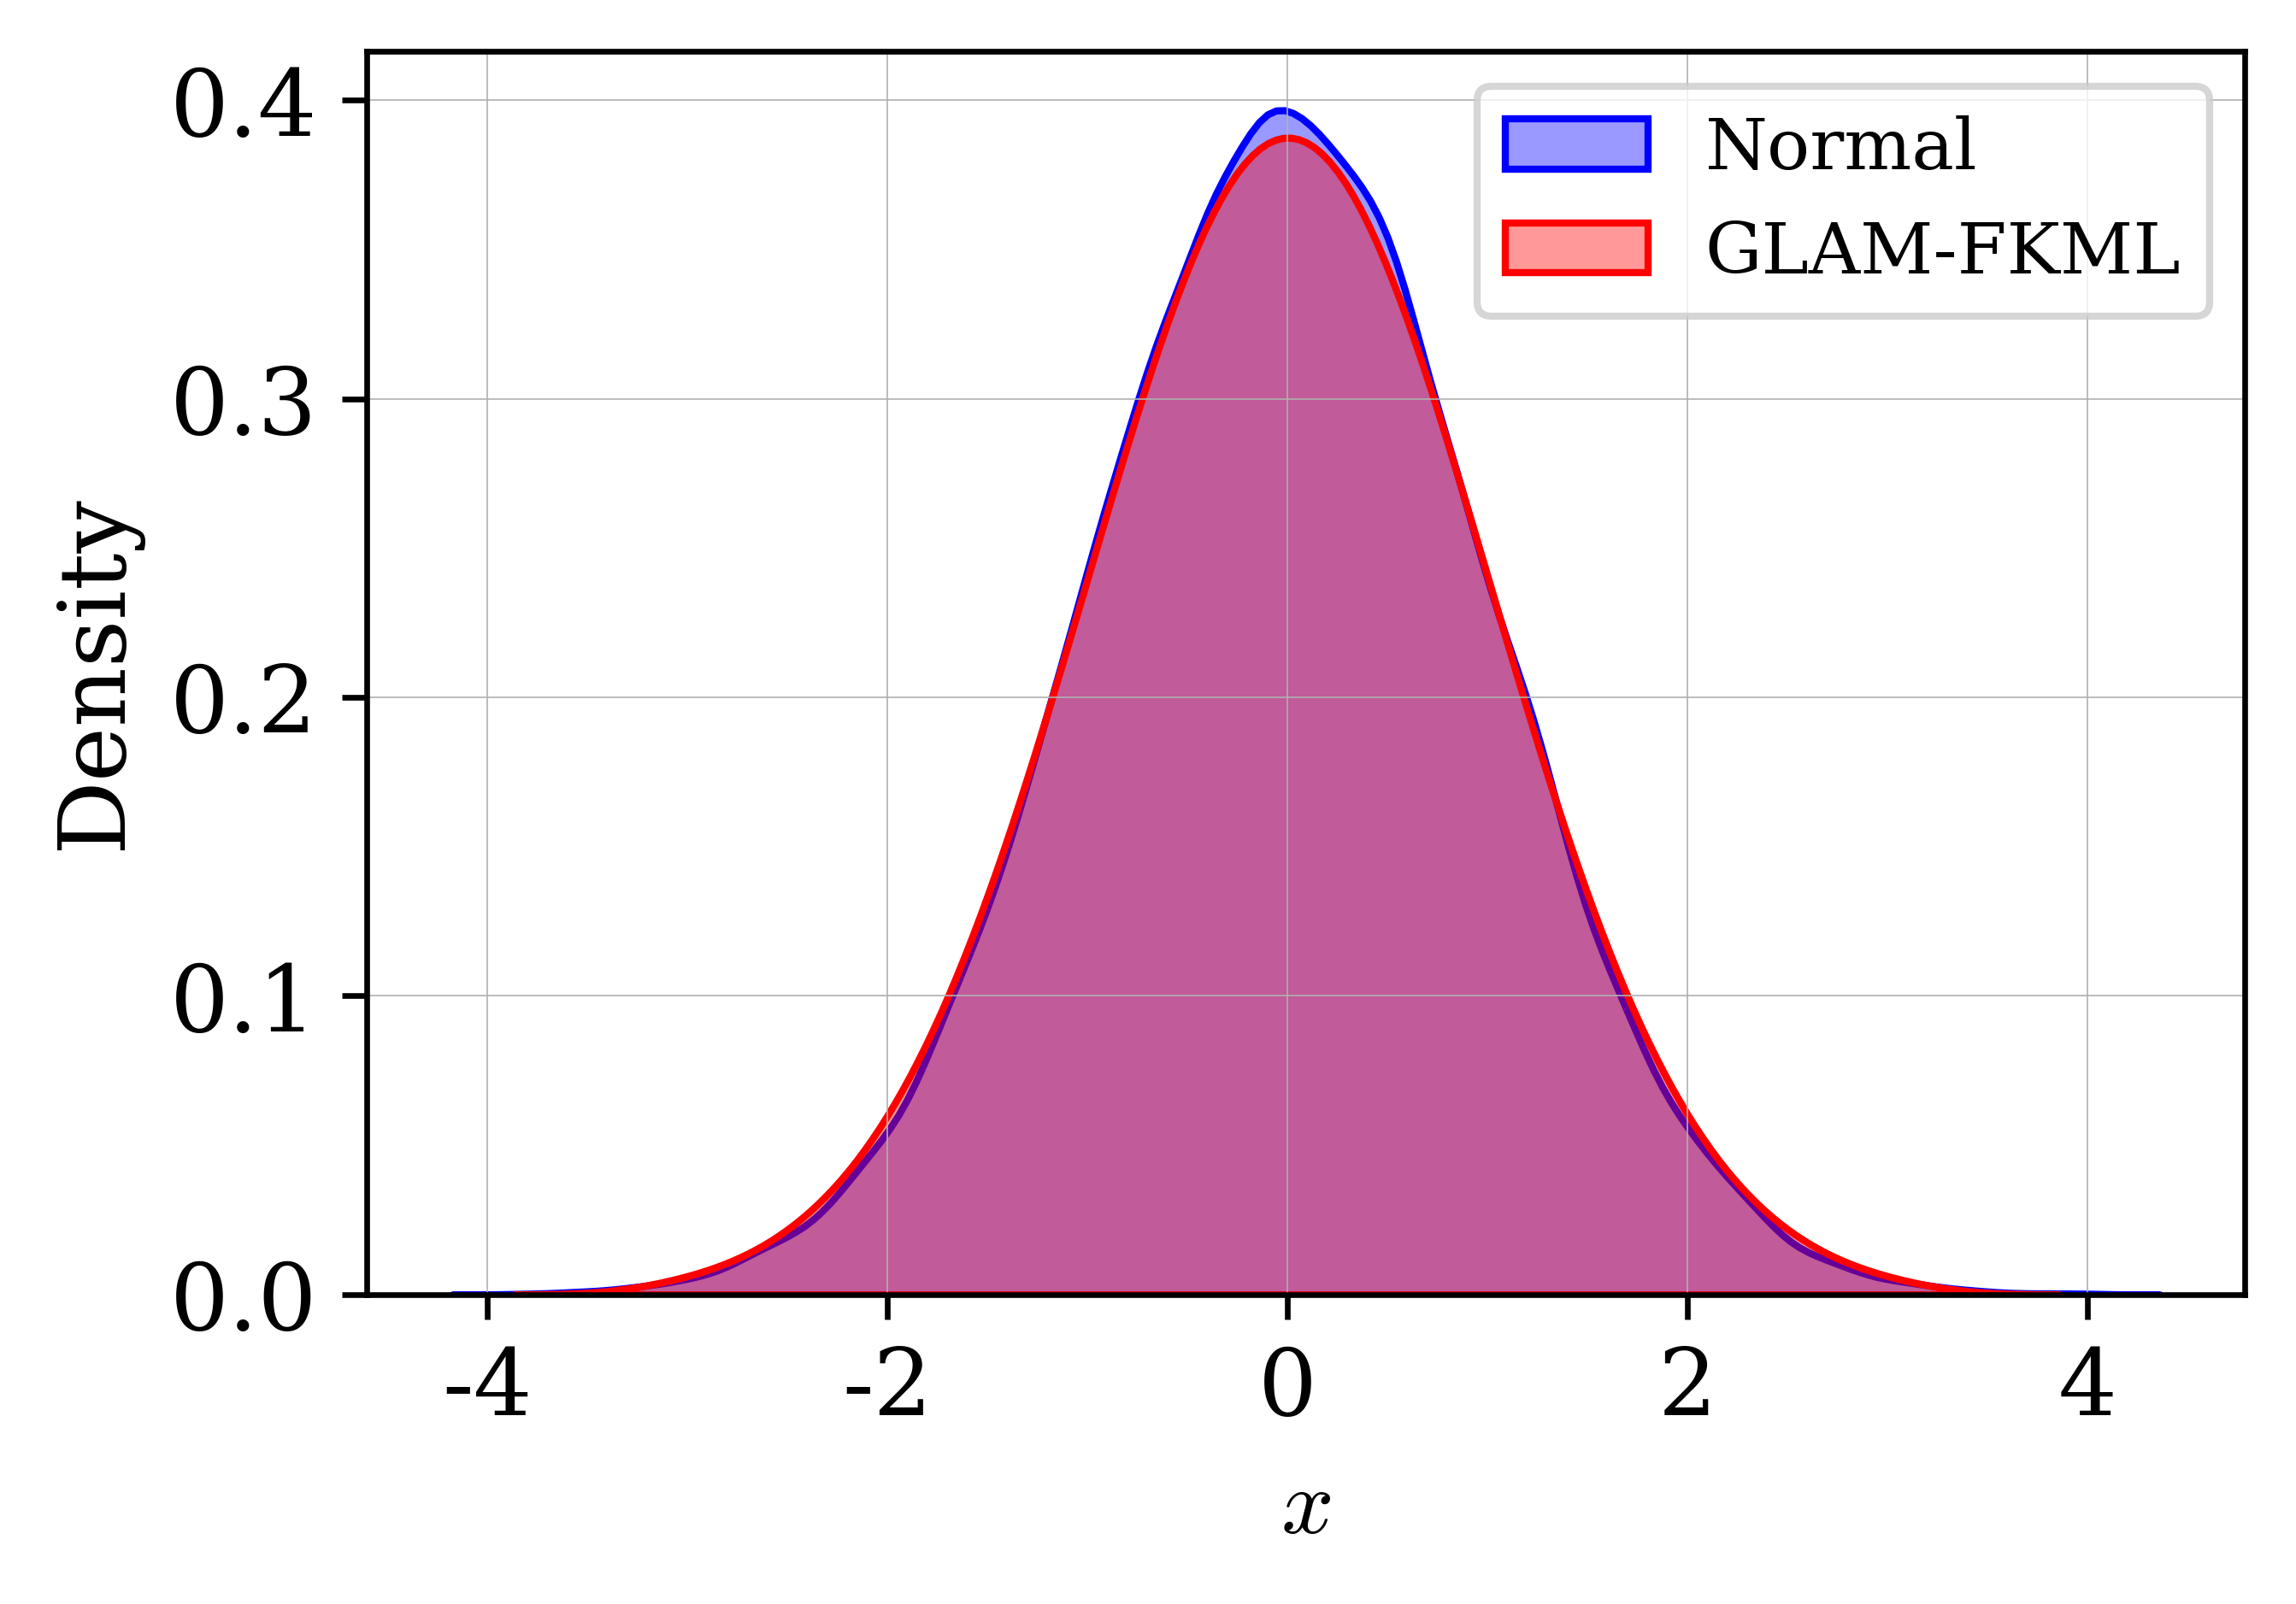
\includegraphics[width=\textwidth]{z_kde_histogram_compare.png}
         \caption{Normal distribution}
         \label{fig:fit_normal}
     \end{subfigure}
     \hfill
     % --- Segunda Subfigura (Gumbel) ---
     \begin{subfigure}[b]{0.32\textwidth}
         \centering
         \includegraphics[width=\textwidth]{fig_gumbel.pdf}
         \caption{Gumbel distribution}
         \label{fig:fit_gumbel}
     \end{subfigure}
     \hfill
     % --- Terceira Subfigura (Uniforme) ---
     \begin{subfigure}[b]{0.32\textwidth}
         \centering
         \includegraphics[width=\textwidth]{fig_uniform.pdf}
         \caption{Uniform distribution}
         \label{fig:fit_uniform}
     \end{subfigure}
     
     \caption{Validation of PyGLAM fitting capabilities for different target distributions using GLD emulators.}
     \label{fig:pyglam_fits}
\end{figure}

\subsection{Generate a emulator with Polynomial Chaos Expansion}

Following the methodology proposed by \citet{ZhuSudret2020-GLAMoriginal} and further developments in stochastic surrogate modeling, the Generalized Lambda Distribution (GLD) is coupled with Polynomial Chaos Expansion (PCE) to construct a global emulator. In this framework, the stochastic response of the simulator for any input $\mathbf{X}$ is modeled by a GLD whose parameters $\boldsymbol{\lambda}$ are themselves functions of the input variables.

Given a set of input parameters $\mathbf{X}$ governed by a joint probability density function $f_{\mathbf{X}}(\mathbf{x})$, each component of the GLD parameter vector $\lambda_i$ is approximated by a truncated PCE:

\begin{equation}
\lambda_i(\mathbf{X}) \approx \sum_{\boldsymbol{\alpha} \in \mathcal{A}} a_{i, \boldsymbol{\alpha}} \Psi_{\boldsymbol{\alpha}}(\mathbf{X}), \quad i = \{1, 2, 3, 4\}
\label{eq:pce_lambda}
\end{equation}

where $\Psi_{\boldsymbol{\alpha}}(\mathbf{X})$ are multivariate orthonormal polynomials specific to the input distributions, $a_{i, \boldsymbol{\alpha}}$ are the polynomial coefficients to be determined, and $\mathcal{A}$ is the set of multi-indices defining the truncation scheme (e.g., total degree basis).

The training procedure for the PCE-GLD emulator follows these steps:

\begin{enumerate}
    \item \textbf{Experimental Design:} A set of $M$ sample points $\{\mathbf{x}^{(1)}, \dots, \mathbf{x}^{(M)}\}$ is generated using Latin Hypercube Sampling (LHS).
    \item \textbf{Stochastic Evaluations:} For each sample point $\mathbf{x}^{(j)}$, the original stochastic simulator is executed $N$ times to obtain a local sample set of the response $\mathcal{Y}^{(j)}$.
    \item \textbf{Local GLD Fitting:} The Method of Moments, implemented via PyGLAM with the BFGS optimizer, is used to estimate the optimal local parameters $\hat{\boldsymbol{\lambda}}^{(j)}$ for each $\mathcal{Y}^{(j)}$.
    \item \textbf{PCE Coefficients Estimation:} Using the pairs $\{\mathbf{x}^{(j)}, \hat{\boldsymbol{\lambda}}^{(j)}\}_{j=1}^M$, the PCE coefficients $a_{i, \boldsymbol{\alpha}}$ are computed for each $\lambda_i$.
\end{enumerate}

Once trained, the emulator can instantly provide the complete probability distribution (via the $\lambda$ parameters) for any new input $\mathbf{X}^*$ without requiring new runs of the original stochastic simulator.

\subsection{Time-Dependent Stochastic Emulation}

The carbonation process is inherently time-dependent, requiring the evolution of the depth distribution to be captured throughout the structure's service life. To account for this, the PCE-GLD framework is extended to include time $t$ as a continuous input variable. In this temporal emulation scheme, the GLD parameters $\boldsymbol{\lambda}$ are evaluated at discrete time steps, and a machine learning (ML) surrogate is subsequently trained to map the joint input space of physical variables $\mathbf{X}$ and time $t$ to the distribution parameters.

The dataset for training the temporal emulator is constructed by evaluating the stochastic simulator at $N_t$ discrete time steps $\{t_1, t_2, \dots, t_{N_t}\}$ (e.g., 0, 10, 20, 50, and 80 years). For each time step $t_m$, a set of $M$ samples of the input vector $\mathbf{X}^{(j)}$ is evaluated, yielding the corresponding local GLD parameters $\hat{\boldsymbol{\lambda}}^{(j, m)}$ via the PyGLAM software. The resulting dataset $\mathcal{D}$ is defined as:

\begin{equation}
\mathcal{D} = \left\{ \left( \mathbf{x}^{(j)}, t_m \right), \hat{\boldsymbol{\lambda}}^{(j, m)} \right\} \quad \text{for } j=1,\dots,M \text{ and } m=1,\dots,N_t
\end{equation}

To predict the GLD parameters at any arbitrary time step $t^*$, a multi-output machine learning model is employed. The model learns the non-linear mapping $f: (\mathbf{X}, t) \to \mathbb{R}^4$:

\begin{equation}
\hat{\boldsymbol{\lambda}}(\mathbf{X}, t) \approx \mathcal{M}_{ML}(\mathbf{X}, t; \mathbf{w})
\end{equation}

where $\mathcal{M}_{ML}$ represents the chosen regressor (e.g., Random Forests, Support Vector Regression, or Neural Networks) and $\mathbf{w}$ denotes the optimized hyperparameters. By including the time step as an explicit input, the emulator can interpolate the values of $\{\lambda_1, \dots, \lambda_4\}$ between the simulated years, providing a continuous evolution of the carbonation depth PDF over the entire analysis period.

% Parametrizing the quantile function is equivalent to modeling the inverse probability integral transform. More precisely, a random variable $Y$ with $Q$ as its quantile function and a random variable $Q(U)$ with $U \sim \mathcal{U}(0,1)$ follow the same distribution. Consequently, the PDF $f_Y(y)$ of a random variable $Y$ following a GLD can be calculated through a change of variables as follows:

% \begin{equation}
% f_Y(y) = \frac{f_U(u)}{Q'(u)} = \frac{\lambda_2}{u^{\lambda_3-1} + (1 - u)^{\lambda_4-1}} \mathbb{1}_{[0,1]}(u), \quad \text{with } u = Q^{-1}(y)
% \end{equation}

% where $\mathbb{1}_{[0,1]}(u)$ is the indicator function and $Q'(u)$ denotes the derivative of the quantile function, also known as the quantile density function.




% Na prática, esta última decorre de variáveis aleatórias latentes \( \mathbf{Z}(\omega) \) (definidas sobre o mesmo espaço de probabilidade, com suporte \( \mathcal{D}_Z \subset \mathbb{R}^{M_Z} \)), que são parâmetros internos do simulador não explicitamente considerados como variáveis de entrada.  

% Em outras palavras, um simulador estocástico é construído a partir de um modelo determinístico \( \mathcal{M} \) da seguinte forma:
% \begin{equation}
% \mathcal{M}_S(\mathbf{x}, \omega) = \mathcal{M}(\mathbf{x}, \mathbf{Z}(\omega)).
% \label{eq3}
% \end{equation}

% Para um dado vetor de entrada \( \mathbf{x}_0 \), cada execução do simulador corresponde a uma realização diferente das variáveis latentes \( \mathbf{Z} \), digamos \( \mathbf{z}_0 \equiv \mathbf{Z}(\omega_0) \), e fornece uma realização particular da variável aleatória de saída \( Y_{\mathbf{x}_0} \equiv \mathcal{M}_S(\mathbf{x}_0, \cdot) \).  
% Para caracterizar a distribuição desta variável de saída, devem ser geradas repetições, isto é, múltiplas execuções de \( \mathcal{M}_S \) com o mesmo vetor de entrada \( \mathbf{x}_0 \) e diferentes realizações \(\{\mathbf{z}_1, \ldots, \mathbf{z}_R\}\) das variáveis latentes.  Referir-nos-emos à função densidade de probabilidade de \( Y_{\mathbf{x}_0} \) como a \textit{distribuição condicional da resposta} dado \( \mathbf{x}_0 \).

% Em contraste, ao fixar a realização \(z_0\) e executar o modelo para diferentes entradas, obtém-se uma
% trajetória do simulador, ou seja, uma função (padrão)  \(\mathcal{M}_S(\cdot, \omega_0) : D_X \to \mathbb{R}\). 
% Essa função pode ser obtida na prática redefinindo a semente do gerador de números aleatórios que
% gera as realizações de \(Z\) para cada \(x\). Resumos estatísticos da saída de um simulador 
% estocástico, como valor médio, variância ou quantis, também são funções padrão dos parâmetros de entrada.

 

 